\documentclass[a4paper]{article}

\setlength{\oddsidemargin}{-4mm}
\addtolength{\topmargin}{-1in}
\addtolength{\footskip}{+0.5in}
\addtolength{\textwidth}{+1.5in}
\addtolength{\textheight}{+1in}

\usepackage[utf8]{inputenc}
\usepackage[english]{babel}
\usepackage{listings}
\usepackage{color}
\usepackage{multirow}
\usepackage{rotating}
\usepackage{graphicx}
\usepackage{caption}
\usepackage{amsmath}
\usepackage{subfig}
\usepackage{hyperref}
\hypersetup{linktocpage}
\renewcommand{\familydefault}{cmr}

\title{Practical report of Lab 3 \\
Operation Research Course}
\author{Hong-Nam Hoang, Manh-Ha Nguyen and Xuan-Thu Thi Le}
\date{\today}

\begin{document}
  \maketitle
%  \tableofcontents
%  \newpage

  \definecolor{stringcolor}{rgb}{0.20,0.50,0.20}
  \definecolor{commentcolor}{rgb}{0.40,0.40,0.40}
  \definecolor{keywordcolor}{rgb}{0.50,0.10,0.10}
  \definecolor{idcolor}{rgb}{0.10,0.10,0.50}
  \definecolor{bg}{rgb}{0.95,0.95,0.95}  
  \lstdefinestyle{iizke}{basicstyle=\ttfamily,
                          keywordstyle=*\color{keywordcolor}\bfseries,
                          identifierstyle=\color{idcolor},
                          commentstyle={\color{black}\it},
                          stringstyle={\color{stringcolor}\ttfamily},
                          showstringspaces=false,
                          breaklines=true,
                          numbers=left,
                          numbersep=10pt,
                          stepnumber=1,
                          numberstyle=\small,
                          frame=single,
                          }

  \lstdefinelanguage[]{Click}[]{SQL}{
    morekeywords={elementclass, Counter, InfiniteSource, RateSource, Print, Paint, PaintSwitch, Script}}

%  \section{Introduction - Netlib package}
%   Source: \url{http://qilfau.googlecode.com}.
%    \subsection{File organization}
%    \subsection{Explore the existing code}
%    Some useful functions: \\
%    add\_link(): Add a new link to graph.
  \section{Algorithms of generating random graph}
  \subsection{Regular ring}
  Function: \texttt{topo\_build\_regular\_ring(PGRAPH g)} \\
  Algorithm: Node $i$ is connected to node $(i+1)\%N$, where $N$ is the number of nodes in ring and the ID of node is in range [0, $N$-1]. \\
    \texttt{For each node $s$ in graph $G$; do \\
      $d$ = ($s$+1)\%$N$; \\
      add\_link($G$, $s$, $d$, 0); \\
      done}
  \subsection{Random ring}
  Function: \texttt{topo\_build\_random\_ring(PGRAPH g, int num\_tx)}, where \texttt{num\_tx} is the number of transmitters/receivers in each node.\\
  Algorithm: The first node ID is always 0. We find a sequence of nodes by selecting node ID randomly so that it is not matched to any nodes selected before and new link is also not assigned before. This condition in some cases is difficult to achieve (for small number of nodes but high value of $\Delta$) and take long time (just for building the ring), so we only try this condition in $10*N$ steps. And then we make a ring from this sequence.\\
  \texttt{Do looping the following procedure num\_tx times:\\
  int seq[N]; \\
  seq[0] = 0; \\
  for i from 1 to N - 1; do \\
  \indent src = seq[i-1]; \\
  \indent ntries = 10 * N; // maximum number of tries to find a good link \\ 
  \indent step\_R: dest = random(1, N-1); // generate random number from 1 to N-1 \\
  \indent ntries--;\\
  \indent if (ntries >= 0) and (link (src, dest) was assigned in graph G); then \\
  \indent\indent repeat step\_R;\\
  \indent if dest is matched in the list seq then \\
  \indent\indent  repeat step\_R; \\
  \indent end-if\\
  \indent add dest to list seq; \\
  \indent if there is no link (src, dest) then \\
  \indent\indent  add\_link (G, src, dest, 0); \\
  \indent end-if\\
  done}
  \subsection{Erd\"{o}s-R\'{e}nyi random graph}
  Function: \texttt{PGRAPH build\_initial\_solution(PGRAPH G, double prob, int iter\_start)}, if (\texttt{iter\_start = 1}) then each edge is included in the graph with probability \texttt{prob} independent from every other edge\\
  Algorithm: \\
  \texttt{
  for all $i \in [1,N], j \in [1,N]$; do\\
  \indent if $j \neq i$ and link (i,j) is not added in graph G; then \\
  \indent\indent Generate uniform random value $p \in [0,1]$\\
  \indent\indent if ($p < prob$) then add\_link (G, i, j, 0); end-if\\
  \indent end-if\\
  done}
  \subsection{Greedy heuristic}
  Function: \texttt{PGRAPH build\_greedy(PGRAPH G, int num\_tx)}\\
  This function is used to build the initial solution based on the idea of greedy heuristic.\\
  Algorithm: \\
  \texttt{
  Step 1: Find $t_{max} = \max (t^{ij})$ \\
  Step 2: If ($t_{max} == 0$) then goto Step 4;\\
  Step 3: \\
  \indent If ($\delta_O^s > 0$) and ($\delta_I^d > 0$); then\\
  \indent \indent add\_link(g, s, d, 0);\\
  \indent \indent  $\delta_O^s$--;\\
  \indent \indent  $\delta_I^d$--; \\
  \indent end-if\\
  \indent $t^{sd} = 0$;\\
  \indent goto step 1;\\
  Step 4: Assign links among remaining Tx and Rx.  
  }
  \section{Experimental results of LTD problem}
  \subsection{Number of node and maximum traffic}
  We do experiment with random ring topology. Number of nodes ($N$) is from 10 to 70, number of transmitters/receivers ($\Delta$) is from 1 to 5. In each pair of $N$ and $\Delta$, we do the test with 10 different values of seed. We use uniform traffic matrix, in which the traffic sent from any source to any destination is a uniform random variable in the range [0.5;1.5].
    \begin{center}
    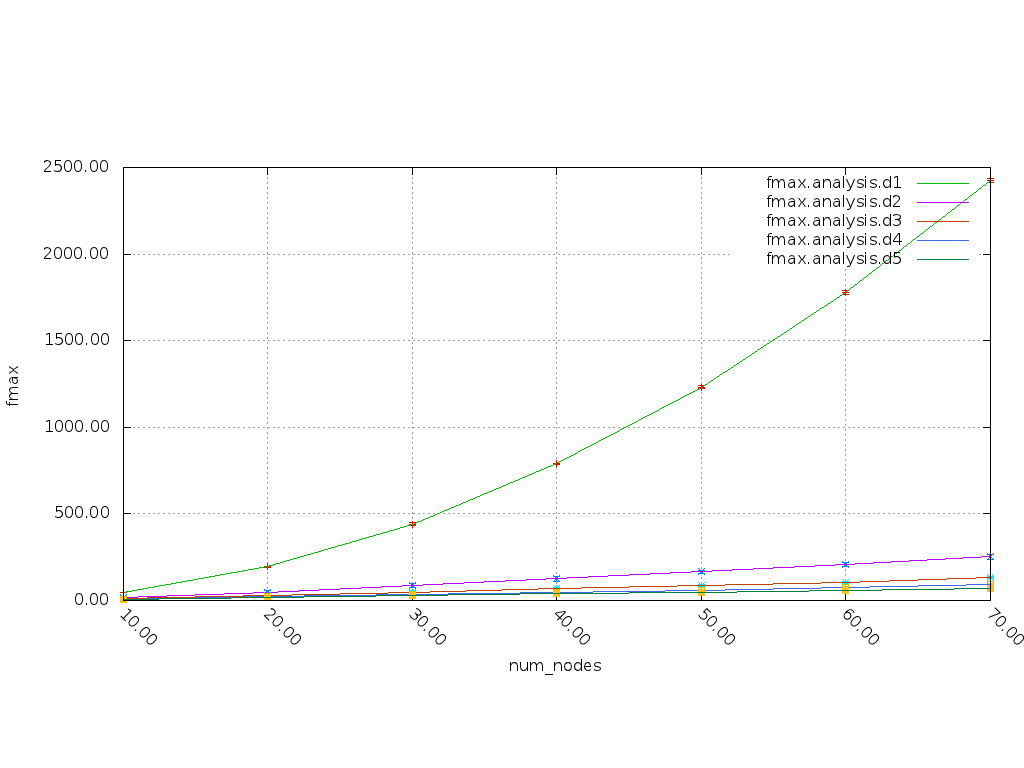
\includegraphics[width=0.8\textwidth]{random-ring-results/plot_n_f.png}
    \captionof{figure}{Maximum traffic over number of nodes (fixed delta)}
    \label{fig:plot-n-f}
    \end{center}
  Observations:
  \begin{itemize}
  	\item With fixed value of $\Delta$, when number of node increases, maximum traffic is increases. The reason is that the traffic from one node is increased (and also carrying traffic for other nodes), but the number of link (out and in) per node does not change, so the traffic per link is increased.
  	\item With fixed value of nodes, when $\Delta$ increases, maximum traffic decreases. The reason is that a node will have more choices ($\Delta$) of routing the traffic, and then reduce the traffic aggregated in a link. 
  	\item In a simple ring ($\Delta = 1$), traffic increases faster than other rings with $\Delta > 1$. 
  	\item Although larger value of $\Delta$ gives a better result of maximum traffic on link, but it is worth to choose $\Delta \in \{2,3\}$ than other values. Clearly, it is much better than case of $\Delta = 1$, but no much less efficient than $\Delta \in \{4, 5\}$ (figure \ref{fig:plot-d-f-ring}).
  	\item In case of small number of node ($N = 10$), $\Delta = 1$ is good enough.
  \end{itemize}
  \subsection{Number of transmitters/receivers and maximum traffic}
  We have the same observations with the previous part. Beside that, we also do the same tests with Greedy heuristic: it does not work well in case of small number of Tx/Rx. As shown in figure \ref{fig:plot-d-f-greedy}, this heuristic cannot guarantee the connectivity of graph ($f_{max}=0$) in case of $N=40,50,60,70$.
    \begin{center}
    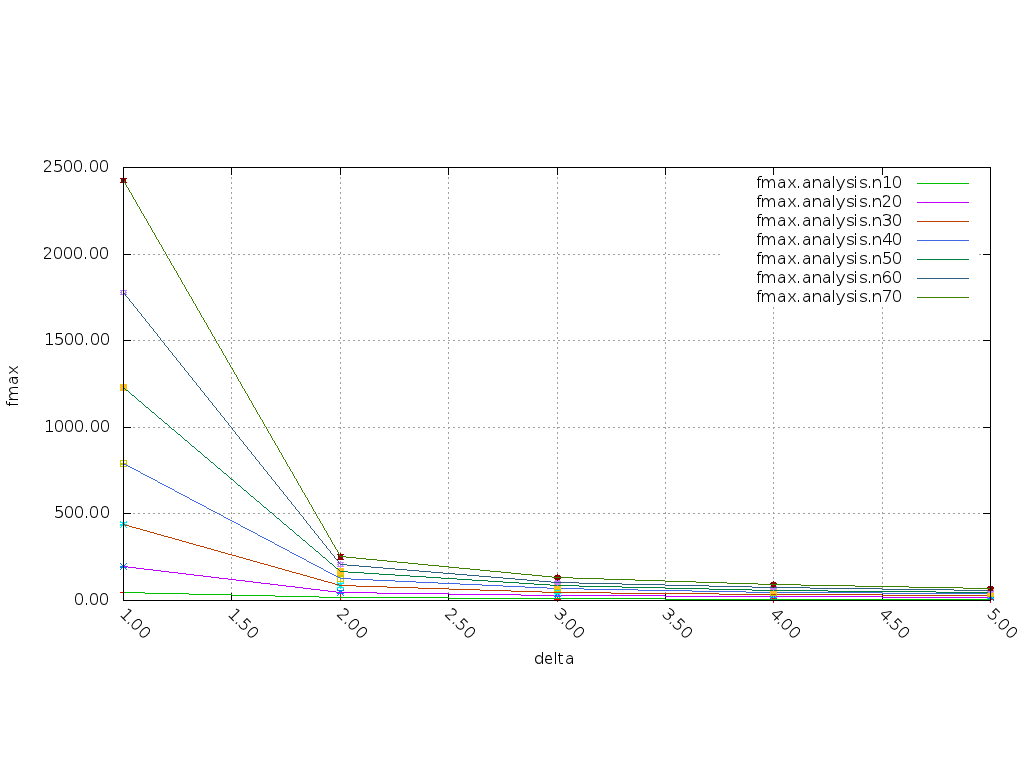
\includegraphics[width=0.8\textwidth]{random-ring-results/plot_d_f.png}
    \captionof{figure}{Maximum traffic over delta (with fixed number of nodes) using Random Ring topology}
    \label{fig:plot-d-f-ring}
    \end{center}
    \begin{center}
    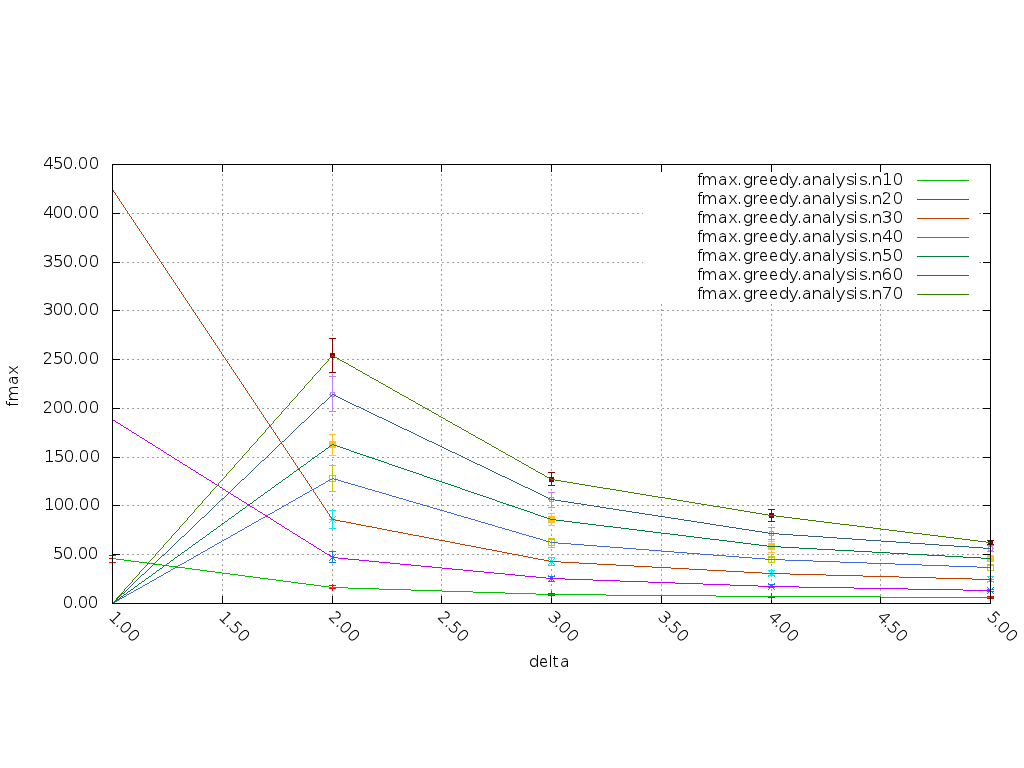
\includegraphics[width=0.8\textwidth]{greedy-results/plot_d_f.png}
    \captionof{figure}{Maximum traffic over delta (with fixed number of nodes) using Greedy heuristic}
    \label{fig:plot-d-f-greedy}
    \end{center}

  \subsection{Seed and maximum traffic}
    We do this experiment to understand how many number of value of seed we should use. Topology is random ring. Number of nodes is 20, number of transmitters/receivers is 1 or 5. In all tests, we use the same traffic which is an uniform random matrix. We do 10 times for each tests.

    \begin{center}
    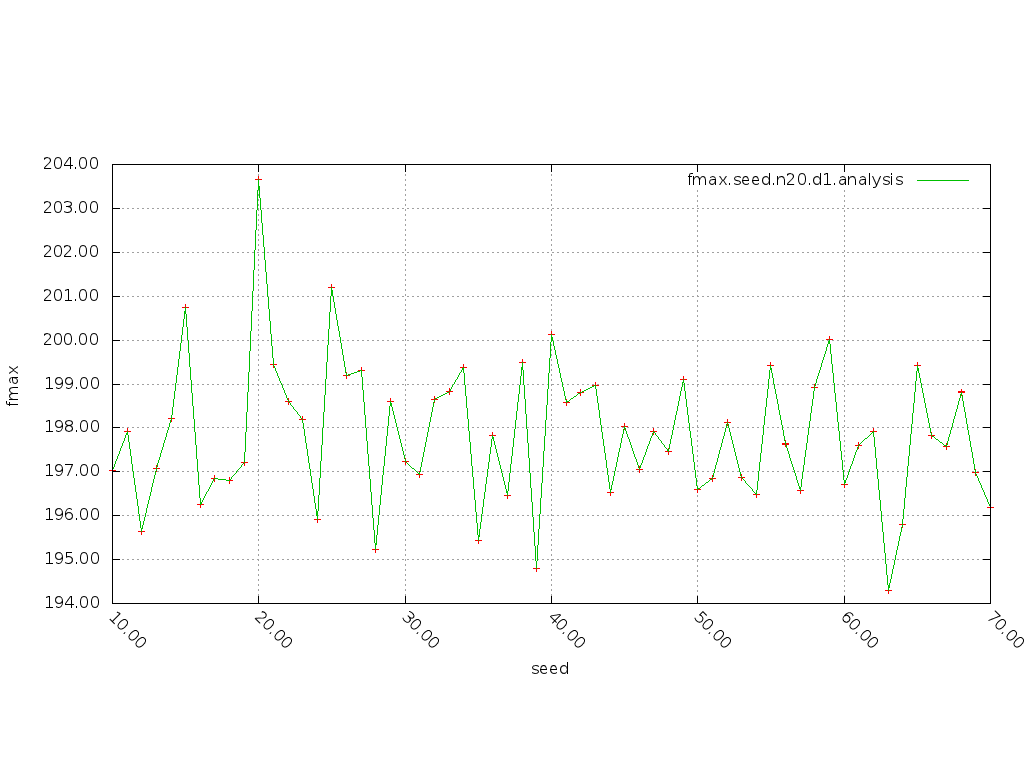
\includegraphics[width=0.8\textwidth]{random-ring-results/plot_s_f.png}
    \captionof{figure}{Maximum traffic over seed ($N=20, \Delta = 1$)}
    \label{fig:plot-s-f-1}
    \end{center}

    \begin{center}
    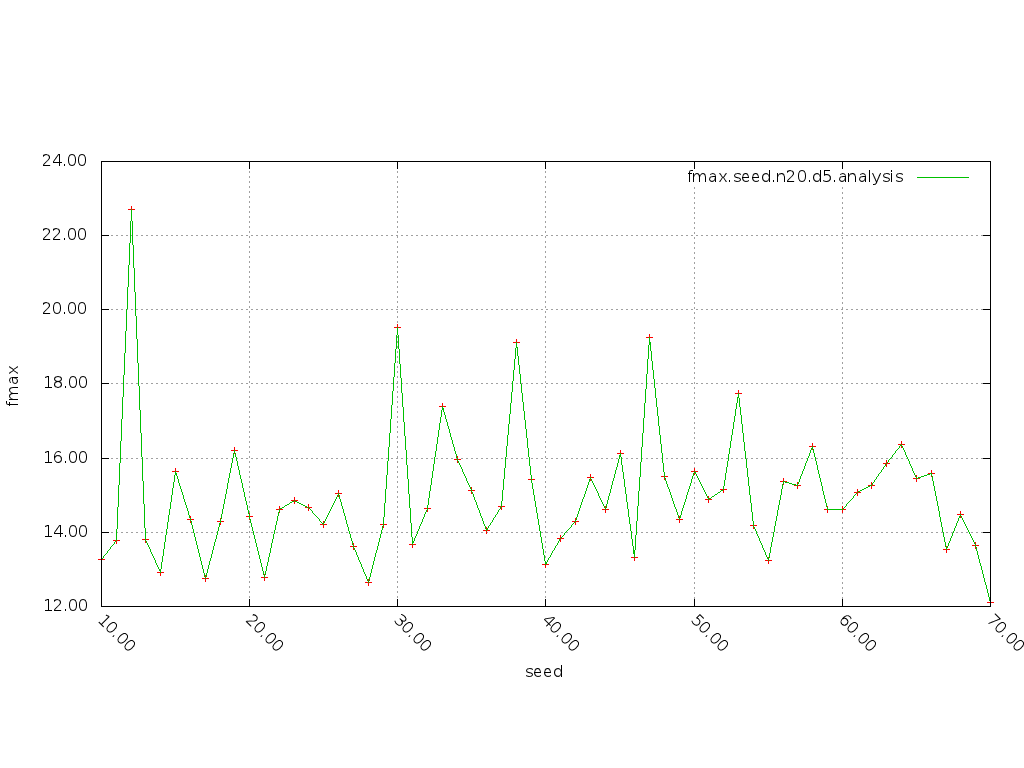
\includegraphics[width=0.8\textwidth]{random-ring-results/plot_s_f5.png}
    \captionof{figure}{Maximum traffic over seed ($N=20, \Delta = 5$)}
    \label{fig:plot-s-f-5}
    \end{center}
  Observations: To get the average value of $f_{max}$, the number of seed should be larger than  or equal to 10. Less than this value, we may get an incorrect average result of $f_{max}$.
  \subsection{Probability and maximum traffic}
  We do experiments with probability applied to ER-Random graph. The probability ($prob$) is changed from 0.1 to 0.9 (step = 0.1). We consider three numbers of nodes ($N$): 20, 40 and 60. The traffic is uniform traffic matrix, in which the traffic sent from any source to any destination is a uniform random variable in the range [0.5;1.5]. In each case of $N$ and $prob$, we iterates 10 times with 10 different value of seed.
    \begin{center}
    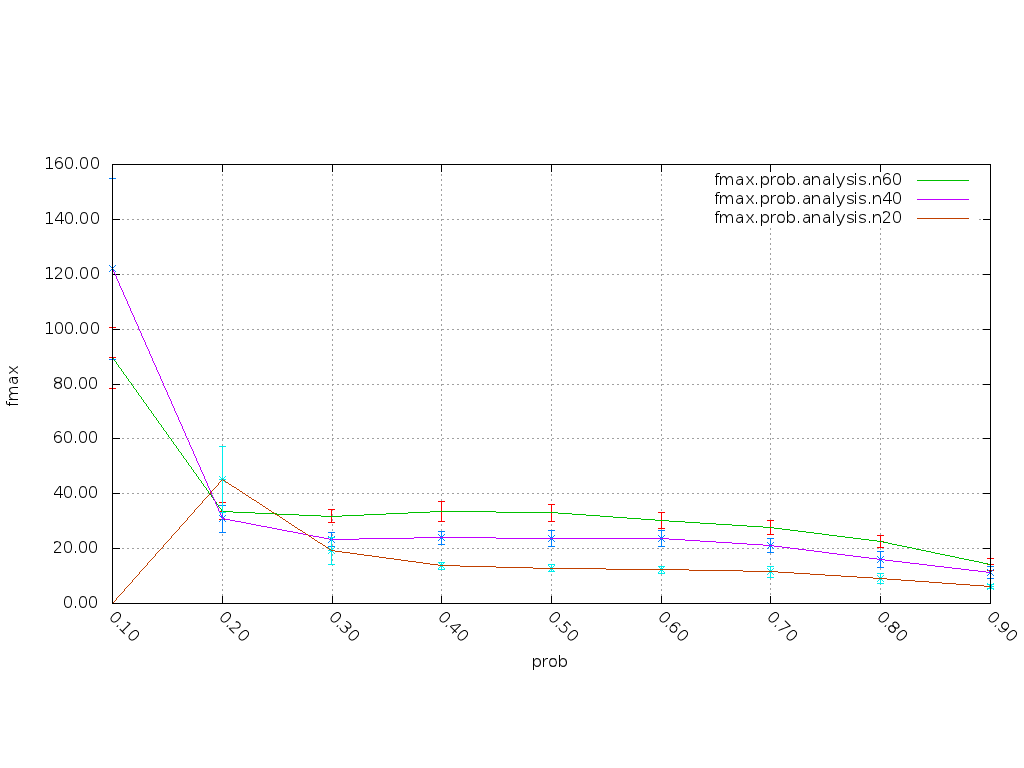
\includegraphics[width=0.8\textwidth]{random-ring-results/plot_pl_f.png}
    \captionof{figure}{Maximum traffic over probability of connectivity (with fixed number of nodes and delta)}
    \label{fig:plot-pl-f}
    \end{center}
    Observations:
\begin{itemize}
  	\item Line n20: when probability = 0.1, maximum traffic is 0, mean that the random graph is disconnected.
  	\item When probability increases, the maximum traffic tends to decrease. The higher probability, the more links are set up, then the maximum traffic is decreased. 
    \item With probability from 0.3 to 0.7: maximum traffic decreases but not much (nearly horizontal line). It can be implied that probability 0.3 or 0.4 is  better than probability 0.7 because generated graphs have less number of links but give the same effect on maximum traffic of link.
    \item With probability from 0.1 to 0.2 in case of line n40, n60 or from 0.2 to 0.3 in case of line n20, the maximum traffic is reduced very much. It is worth to choose probability 0.2 than 0.1 in case of 40 or 60 nodes, and 0.3 than 0.2 in cases of 20 nodes.
    \item With small value of $prob$ (0.1), smaller number of nodes often has larger value of maximum traffic. The reason could be that: with small $prob$, the number of links is small, each node has less number of transmitters/receivers (compared with large $N$), and it is not equal opportunity for every nodes to reach other nodes: some links carry much traffic, some links carry a few traffic, some nodes cannot be reached or disconnected graph (as in case of line n20).
    \item With large value of $prob$, the line n60 is above n40 and n20, but the distances among these line is small.
    \end{itemize}
    
\section{Experimental results on Wavelength Assignment problem}
We do experiments with random ring and ER random graph topology. Number of nodes is from 10 to 70 (step of 10 units). Number of requests is from 10 to 70 (also step of 10 units).
\subsection{Number of nodes and maximum number of wavelength}
    \begin{center}
    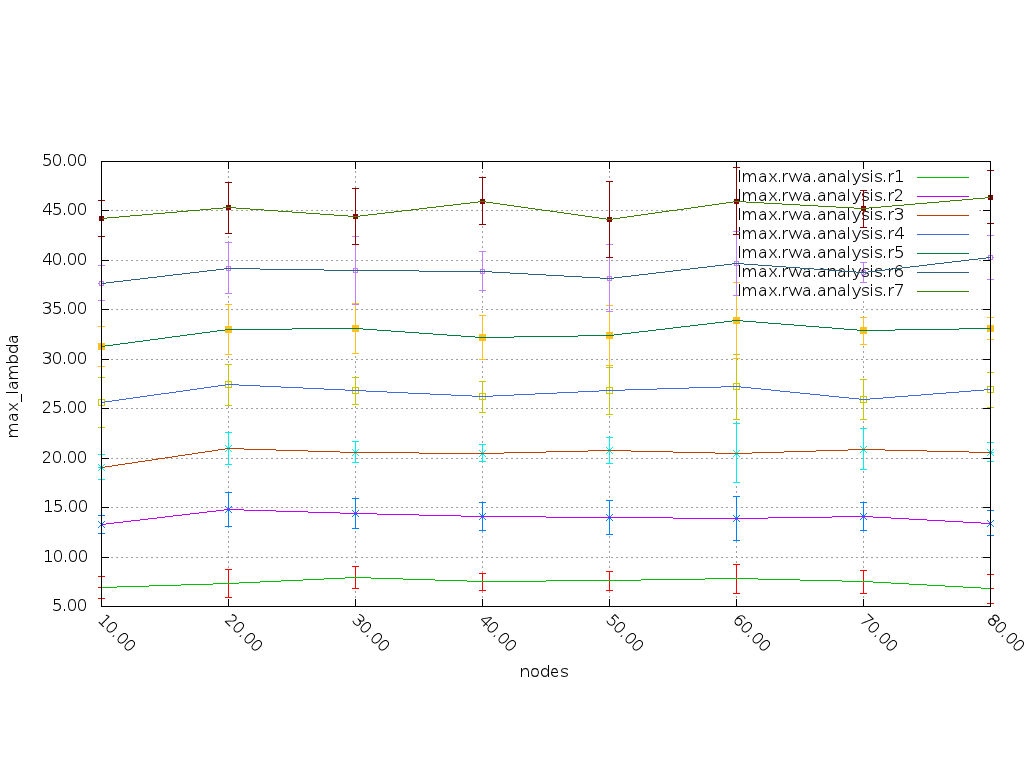
\includegraphics[width=0.8\textwidth]{rwa-ring-results/plot_rwa_n_l.png}
    \captionof{figure}{Maximum number of wavelength over number of nodes (Ring topology, and number of requests is from 10 to 70)}
    \label{fig:plot-rwa-ring-n-l}
    \end{center}
Ring topology (figure \ref{fig:plot-rwa-ring-n-l}):
\begin{itemize}
  \item In the same number of nodes, if number of requests increases then maximum number of wavelengths increases.
	\item In the same number of requests, number of nodes does not make a large effect on maximum number of wavelength. Because of Ring topology, one node has only two directions to reach others, so the number of requests aggregated in the same link is nearly the same even if we increase the number of nodes.
\end{itemize}

    \begin{center}
    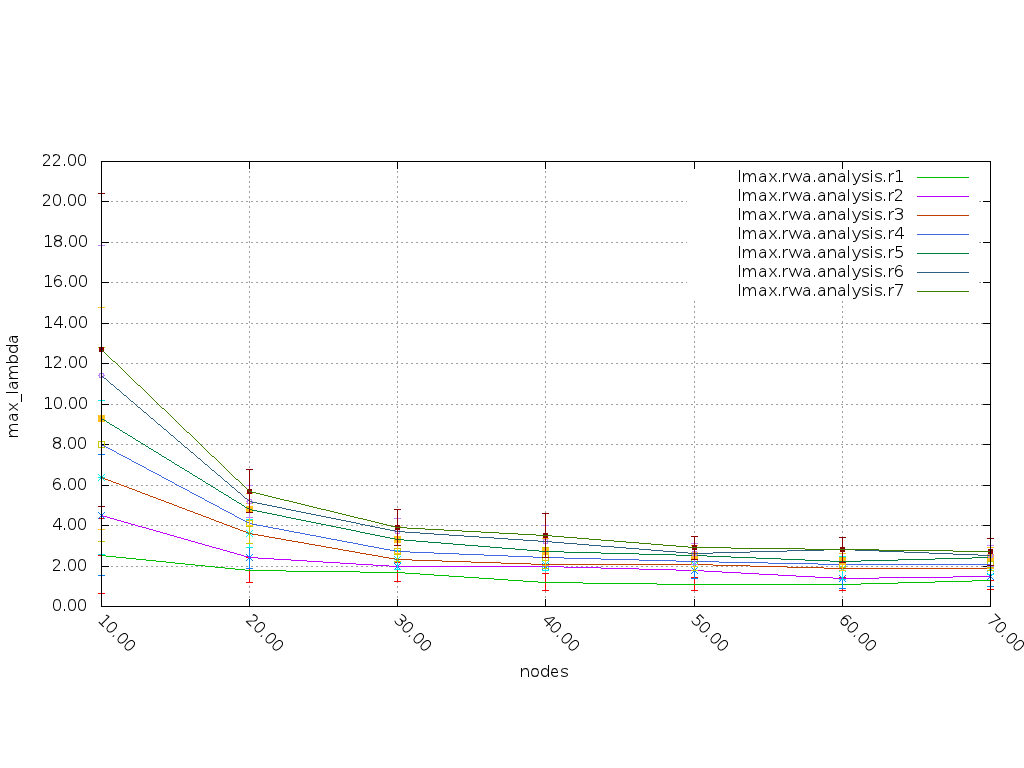
\includegraphics[width=0.8\textwidth]{rwa-prob-results/plot_rwa_n_l.png}
    \captionof{figure}{Maximum number of wavelength over number of nodes (ER random graph topology (probability 0.3), and number of requests is from 10 to 70)}
    \label{fig:plot-rwa-prob-n-l}
    \end{center}

ER random graph topology (figure \ref{fig:plot-rwa-prob-n-l}):
\begin{itemize}
	\item In the same number of nodes, if number of requests increases, then maximum number of wavelength increases.
	\item In the same number of requests, maximum number of wavelength decreases when number of node increases. Because number of links ($O(N^2)$) is also increases, there is a large opportunity to assign each requests on to separating paths.
	\item Maximum number of wavelength decreases very much when number of nodes increases from 10 to 20. Maximum number of wavelength is from 2 to 4 in other cases of number of nodes.
\end{itemize}

\subsection{Number of requests and maximum number of wavelength}
We have the same observation as in previous part (Number of nodes and maximum number of wavelength). In figure \ref{fig:plot-rwa-prob-n-l}, there is a large variance of line n10. We check and recognize the problem of disconnected graph. With $prob = 0.3, N = 10$, it can create a disconnected graph which the returned value of maximum number of wavelength is 0 (these cases should be removed before calculating the mean and variance, and the reason we do not do it is time).
    \begin{center}
    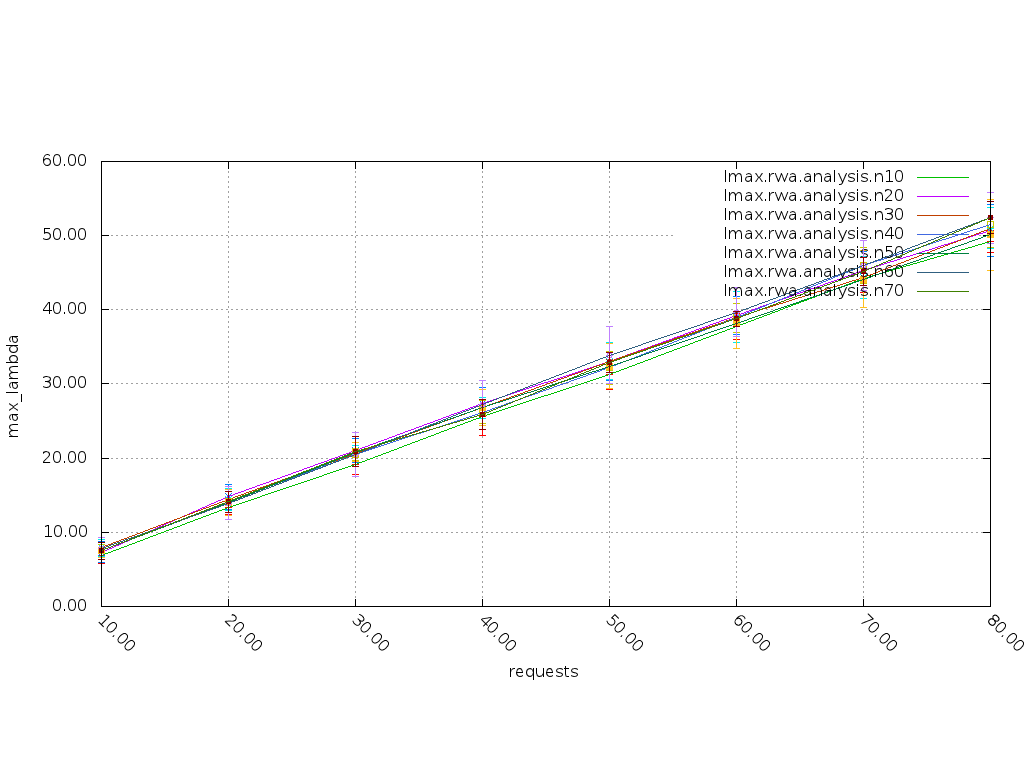
\includegraphics[width=0.8\textwidth]{rwa-ring-results/plot_rwa_r_l.png}
    \captionof{figure}{Maximum number of wavelength over number of requests (Ring topology, and number of nodes is from 10 to 80)}
    \label{fig:plot-rwa-ring-n-l}
    \end{center}

    \begin{center}
    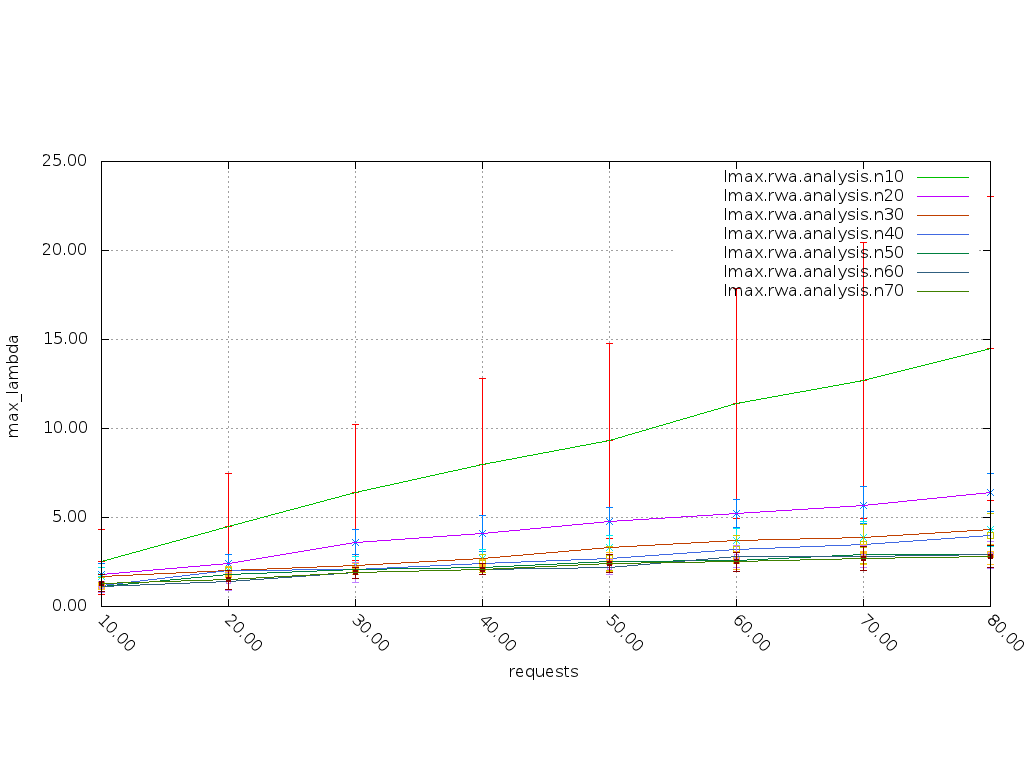
\includegraphics[width=0.8\textwidth]{rwa-prob-results/plot_rwa_r_l.png}
    \captionof{figure}{Maximum number of wavelength over number of requests (ER random graph topology (probability 0.3), and number of nodes is from 10 to 80)}
    \label{fig:plot-rwa-prob-n-l}
    \end{center}

\subsection{Probability and maximum number of wavelength}
We do experiment with fixed number of requests (40), probability from 0.1 to 0.9 (step 0.1). We consider three numbers of node: 20, 40 and 60.
    \begin{center}
    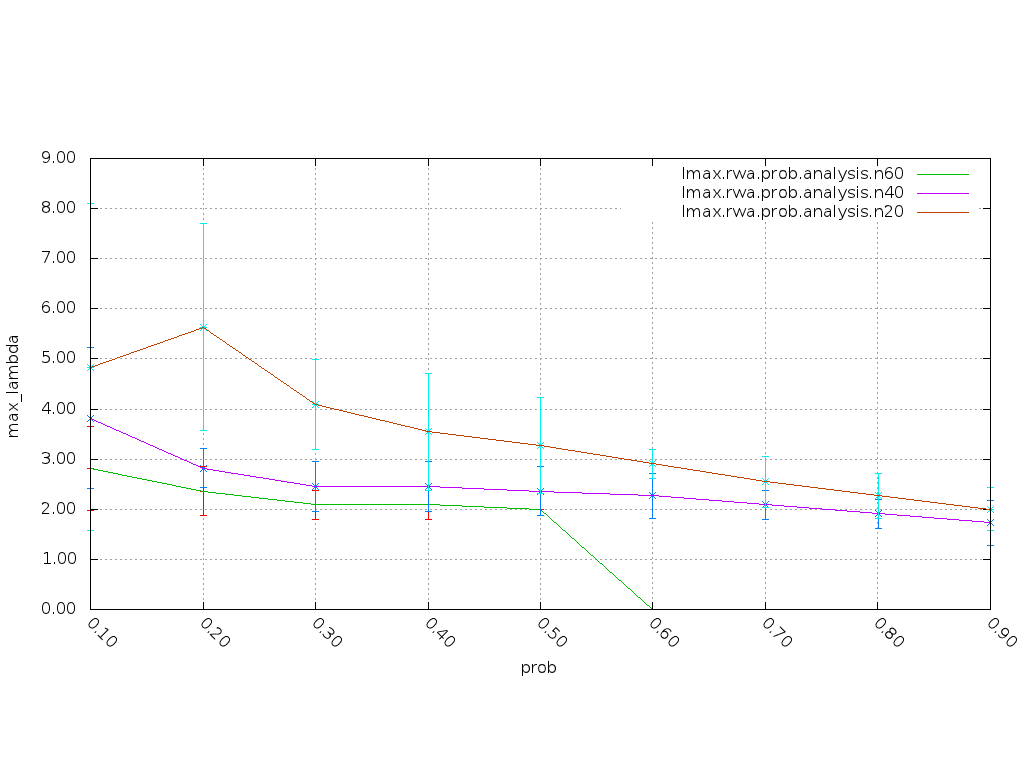
\includegraphics[width=0.8\textwidth]{rwa-prob-results/plot_rwa_pl_l.png}
    \captionof{figure}{Maximum number of wavelength over probability (ER random graph topology, and number of requests is 40)}
    \label{fig:plot-rwa-prob-l}
    \end{center}
\begin{itemize}
	\item Line n60 comes to 0 in cases of probability larger than 0.6. It is because of limitation of memory for simulating program. Our simulation only supports maximum 1800 arcs (directed links), while in the case of 60 nodes and probability 0.6, we may need around 2100 directed links.
	\item In most of cases, when probability is increased (meaning that number of links also is increased), the maximum number of wavelength is decreased.
	\item In case of 20 nodes, the maximum number of wavelength is not stable (high variance). It means that the distribution of requests on graph and topology make a large effect on number of wavelength. 
\end{itemize}
\end{document}
